\section{Implementácia algoritmu}
\label{kap:4}

Kým v predošlej kapitole (kap. \ref{kap:3}) sme si v jednoduchosti vysvetlili ako budeme pristupovať ku plánovaniu trajektórie pri jednotlivých kinematických štruktúrach a opísali sme si konfiguračný priestor pre jednotlivé štruktúry, v tejto kapitole si bližšie vysvetlíme, čo bolo potrebné implementovať do pôvodného kódu aby vyššie spomenuté prístupy fungovali.

Ukážeme si fundamentálne funkcie, na ktorých stojí náš algoritmus a vysvetlíme si ich úlohy a prístup, ktorý sme pri ich implementácii zvolili.
 



\subsection{Vizualizácia}

Pre potreby vývoju nášho algoritmu bolo v prvom rade potrebné vytvoriť vizualizáciu prenášaného objektu v priestore. Pôvodné riešenie uvažovalo len hmotný bod, ktorého pohyb v priestore sa dá jednoducho zobraziť v grafe. Pri našom probléme má však prenášaný objekt svoj, tvar, rozmery a orientáciu v priestore. Z toho dôvodu bola vytvorená vizualizácia, ktorá nám zobrazuje priemet pracovného priestoru robota v osiach $ x $, $ y $ (obr. \ref{OBRAZOK 4.1}). Obsahuje prenášaný predmet, prekážku, ktorá predstavuje stĺp, na ktorom je robotické rameno uchytené  v prípade plánovania trajektórie v kĺbovom priestore aj samotné robotické rameno. Pracovný priestor spolu s prekážkami a objektom sme vizualizovali v mierke  1 $mm$ = 1 $pixel$. 

\begin{figure}[h]
	\centering
	\fbox{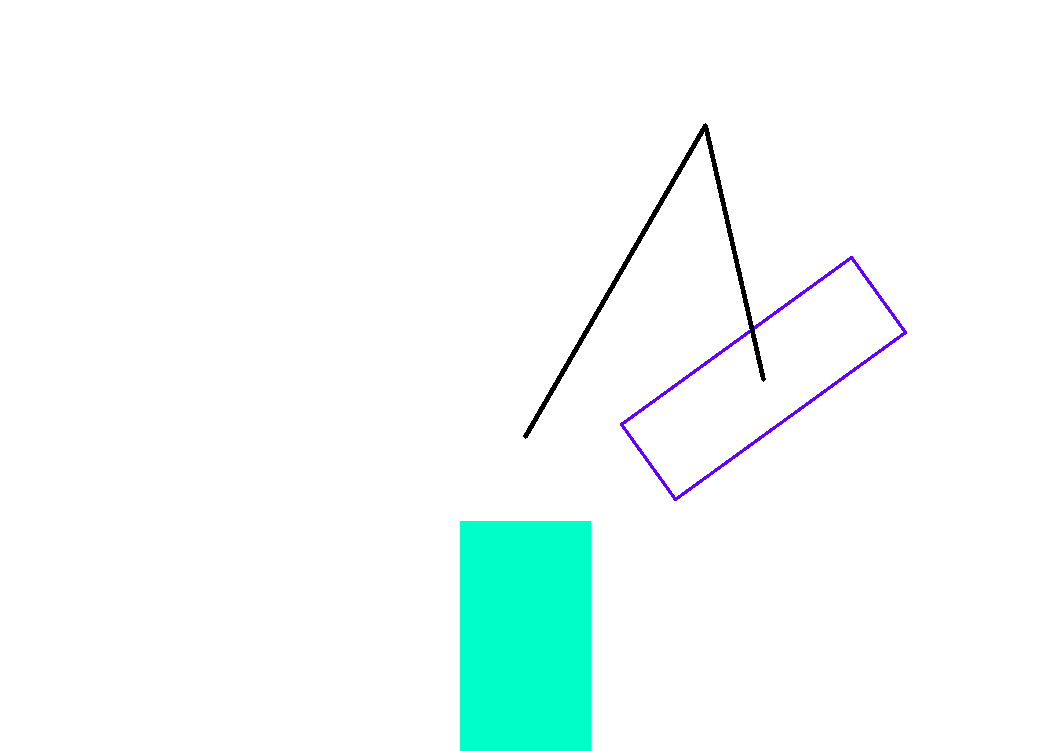
\includegraphics[width=100mm]{img/Vizualizacia.png}}
	\caption{Vizualizácia pracovného priestoru} \label{OBRAZOK 4.1} 
	\label{fig:border}
\end{figure} 

Táto vizualizácia spĺňala v prvom rade kontrolnú funkciu, či vygenerovaná trajektória spĺňa dané požiadavky - sa objekt pri pohybe vyhýba prekážkam a nevychádza z pracovného priestoru.

Prenášaný objekt sme si vizualizovali ako obdĺžnik. Ide o univerzálny geometrický tvar najlepšie odpovedajúci  väčšine tovaru, ktorý by sa mohol v sklade nachádzať. Takmer každá krabička alebo iný objekt sa nám do roviny $ xy $ premietne práve ako obdĺžnik. Objekt sme teda definovali pozíciou jeho stredu, výškou, šírkou a uhlom otočenia. 

Pre vypracovanie tejto časti sme využili knižnicu openCV.

\subsection{Objekt v kolízii}
Hmotný bod prenášaný priestorom má v porovnaní s objektom veľkú výhodu práve v tom, že vieme presne povedať kde v priestore sa nachádza. Tým pádom vieme jednoducho určiť , či je v kolízii s prekážkami alebo opustil pracovný priestor. Pri objekte vieme takýmto spôsobom kontrolovať len jeden jeho bod, ktorým je definovaný a to je v našom prípade jeho stred. Úlohu kontroly kolízie objektu s prekážkami to teda výrazne komplikuje aj vzhľadom na to, že náš objekt mení v priestore aj svoju orientáciu. 

Preto bolo potrebné vytvoriť funkciu, ktorej úlohou bude zistiť či sa náš objekt v danej konfigurácii nenachádza v kolízii alebo neopustil pracovný priestor robota. Touto funkciou je $ collision\_check() $. Ide o základnú funkciu na ktorej stojí celý náš algoritmus a je identická pre všetky kinematické štruktúry. Pracuje v kartézskom súradnicovom systéme. Na základe vstupných údajov, ktorými sú pozícia stredu objektu - súradnice $ x $ a $ y $, rozmery objektu - šírka a výška, a natočenie objektu nám vráti informáciu o tom či sa objekt nachádza v bezkolíznej pozícii. 

\begin{figure}[h!]
	\centering
	\fbox{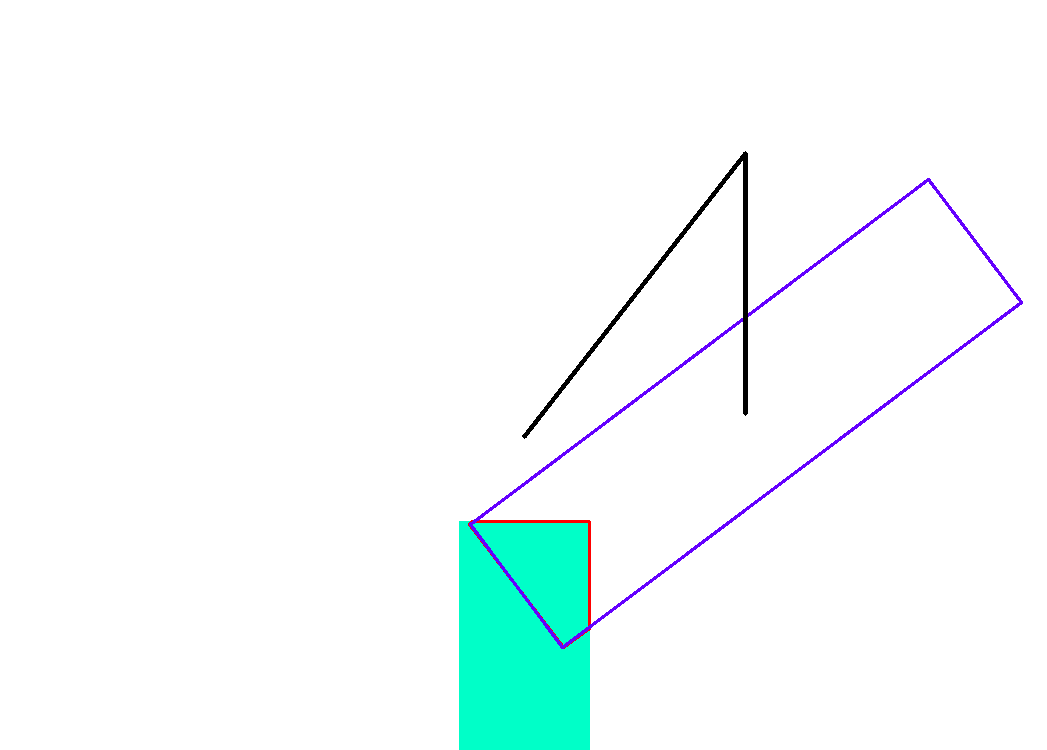
\includegraphics[width=100mm]{img/Kolizia.png}}
	\caption{Objekt v kolízii} \label{OBRAZOK 4.2} 
\end{figure} 

Pre kontrolu kolízie objektu s prekážkami v priestore sme použili knižnicu shapely. Pomocou jej funkcií sme boli schopní na základe parametrov objektu získať pozíciu jeho rohov v priestore a tiež overiť prienik 2 objektov - prenášaného a prekážky, čo nám slúžilo na zistenie kolízie(obr. \ref{OBRAZOK 4.2} ).

Do tejto funkcie sme zahrnuli kontrolu situácie, že prenášaný objekt opustí pracovný priestor robota. Keďže nevieme zaručiť, že priestor mimo pracovné priestoru robota bude voľný, treba ho považovať za obsadený. V prípade, že objekt opusti pracovný priestor je táto konfigurácie tiež považovaná za kolíziu. 
 
\subsection{Overenie dosiahnuteľnosti pozície}

Generovanie trajektórie prebieha v krokoch, kedy sú postupne generované nové konfigurácie alebo inak povedané pozície, ktorými objekt prechádza od počiatku k cieľu (kapitola \ref{kap:2.1}). Prvým krokom je určiť, či sa vygenerovaný nachádza v bezkolíznej konfigurácii, k čomu slúži funkcia $ collision\_check() $. Druhým krokom je zistiť, či sa objekt z bodu, v ktorom sa práve nachádza dokáže dostať do nového bodu, ktorý bol vygenerovaný. Ak by ho objekt z danej pozície nemohol dosiahnuť napr. kvôli prekážke v ceste, tento bod nemôže byť pridaný do generovaného stromu. V prípade hmotného bodu ide o priame spojenie 2 bodov priamkou. Ak sa priamka pretína s prekážkou tak táto pozícia nie je dosiahnuteľná. 

Pri objekte treba uvažovať jeho pohyb v priestore.  Každá pozícia, ktorou objekt pri danom pohybe prejde musí byť bezkolízna. Na obrázkoch \ref{OBRAZOK 4.4} a \ref{OBRAZOK 4.5} môžeme vidieť porovnanie medzi pracovným a konfiguračným priestorom.  Kým v konfiguračnom priestore je pohyb opísaný priamkou v trojrozmernom priestore, v pracovnom priestore ide o pohyb obdĺžnika, kedy sa menia jeho pozícia v osiach $ x $, $ y $ aj uhol natočenia.

\begin{figure}[h!]
	\centering
	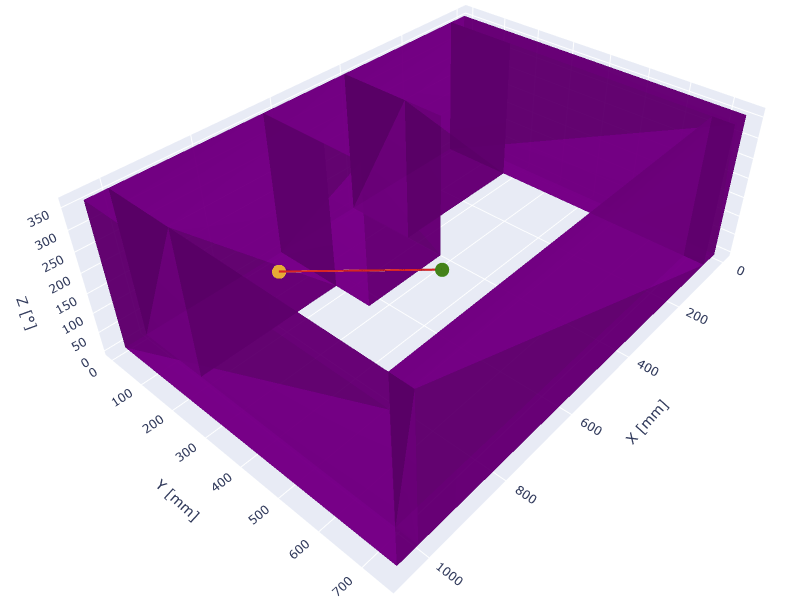
\includegraphics[width=120mm]{img/Path_sampling-Searchspace.png}
	\caption{Spojenie 2 bodov v konfiguračnom priestore} \label{OBRAZOK 4.4} 
\end{figure} 

\begin{figure}[h!]
	\centering
	\fbox{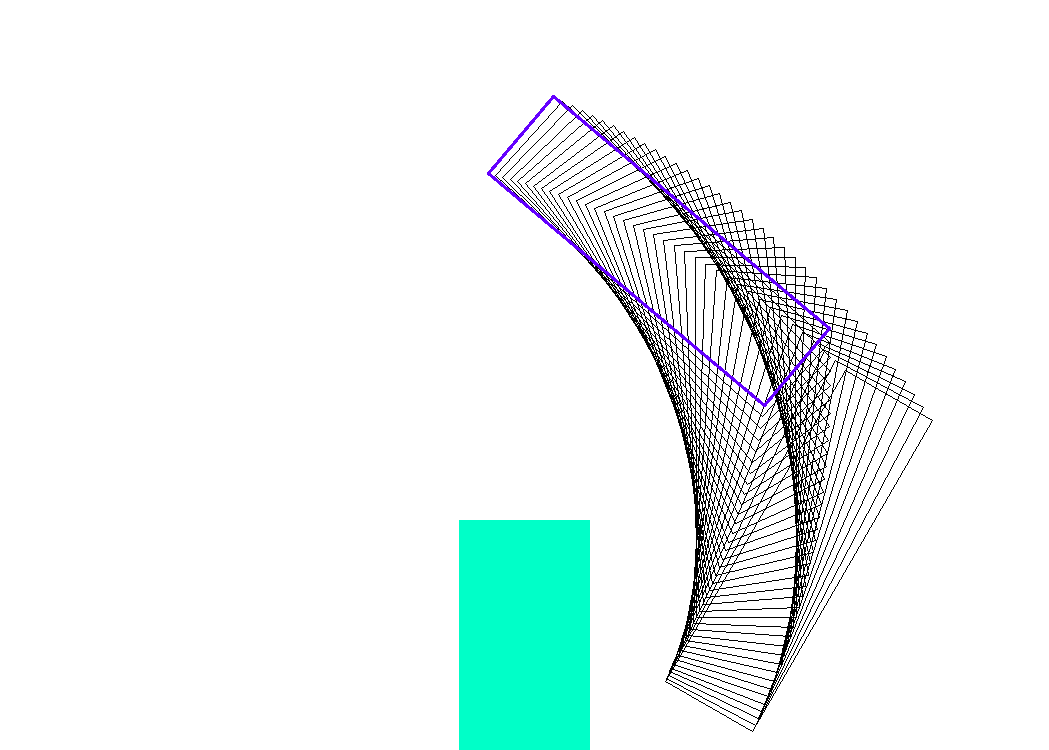
\includegraphics[width=100mm]{img/Path_sampling3D.png}}
	\caption{Pohyb objektu v pracovnom priestore} \label{OBRAZOK 4.5} 
\end{figure} 


Pre simuláciu pohybu v priestore sme použili lineárne vzorkovania. Poznáme počiatočnú a koncovú pozíciu, ktoré nám definujú pohyb - prejdenú vzdialenosť a smer. Vypočítame si veľkosť úsečky medzi danými 2 pozíciami v konfiguračnom priestore. Na základe nami zvolenej veľkosti vzorky si rozdelím danú uhlopriečku na daný počet vzoriek. Postupne inkrementujeme jednotlivé prvky počiatočnej pozície ($ x $,$ y $,$ uhol $) o hodnotu, ktorá odpovedá veľkosti vzorky v danej osi. Tým dosiahneme prechodové pozície, pričom v každej z nich kontrolujeme, či sa objekt nenachádza v kolízii.  Ak sú všetky prechodové pozície vyhodnotené ako bezkolízne vieme, že daný cieľový bod je dosiahnuteľný.
Túto úlohu zabezpečuje funkcia $ linear\_sampling\_collision\_check()$.

OBRAZOK - linearne vzorkovanie


\subsection{Kontrola dosiahnuteľnosti cieľa}

Ukončovacia podmienka algoritmu býva vo väčšine prípadov určená vzdialenosťou generovaného bodu v strome od cieľovej pozície, keď sa generovaný bod dostane do blízkosti cieľa je vytvorené prepojenie a algoritmus je ukončený. Ďalšou možnosťou je použiť ako ukončovacia podmienku maximálny počet iterácií. Algoritmus prehľadáva priestor až dokým nie je vygenerovaný daný počet bodov a až následne hľadá prepojenie s cieľom. Táto ukončovacia podmienka sa dá použiť napríklad pri RRT*, kedy je počtu iterácií úmerná kvalita výslednej trajektórie. Pri algoritme RRT-connect sú generované 2 stromy a ukončenie algoritmu
nastane pri ich spojení.

V našom algoritme využíva určitú kombináciu jednotlivých prístupov.
Jedným so vstupných parametrov, ktorý si definujeme pri spustení algoritmu je pravdepodobnosť, s ktorou si bude algoritmus v priebehu generovania stromu kontrolovať dosiahnuteľnosť cieľa.  V prípade, že je cieľ z daného bodu dosiahnuteľný je vygenerovaná trajektória a algoritmus je ukončený. Na kontrolu dosiahnuteľnosti cieľa z posledného generovaného bodu nám slúži funkcia $ linear\_sampling\_collision\_check()$.

Z dôvodu jednoduchosti pracovného priestoru (obsahuje len jednu prekážku) vo väčšine prípadov prenášaných objektov bude možné nájsť priame spojenie hneď z počiatočnej do cieľovej pozície. Za účelom zvýšenia rýchlosti výpočtu algoritmu v daných prípadoch si algoritmus hneď na začiatku skontroluje dosiahnuteľnosť cieľa, čím sa preskočí celý proces generovania stromu.

Algoritmu je tiež stanovený maximálny počet iterácií. V prípade dosiahnutia maximálneho počtu iterácií je overená dosiahnuteľnosť cieľa z daného bodu. Ak spojenie neexistuje algoritmus je ukončený a trajektória nebola nájdená.

\subsection{3 stupne voľnosti}



\subsubsection{Kartézsky súradnicový systém}

co sme pridali - preco 
 vizualizacia, collisioncheck, path sampling, ...  
 vyvojove diagramy 
 orezanie konfiguracneho priestoru

\subsubsection{Kĺbový súradnicový systém}
 co sme pridali - preco 
 - FK, IK , vizualizacia, ... 
 vyvojove diagramy 
 orezanie konfiguracneho priestoru

\subsection{2 stupne voľnosti}

 opisat rozdiel medzi 2DOF a 3DOF 
 princip predrotacie
 vyvojove diagramy 

